\chapter{Particles, Waves, and the Energy of Resolution}

\section{Particles or Fields?}

What is particle physics about? Particles---but that answer immediately raises an ancient question. Is nature discrete? Discrete here means that matter comes in separate, indivisible units, not that it is tactful. The Greek word \emph{atom} means indivisible, even though objects now called atoms can be broken apart. For the moment, \emph{particle} will be the generic name for a discrete unit.

The opposing picture is a continuum. Matter is then not a collection of separate pieces but a continuous smear through space. Its natural language is the language of fields. A field is a function of position: the density of a material is a field, and the electric and magnetic fields are fields. The latter determine how charged particles move, but the fields themselves are conceived classically as continuously distributed through space.

The historical order of these ideas should not be pressed too hard. The sequence is useful because it displays the logic of the argument, not because it supplies a dependable chronology. The particle vocabulary includes atoms, molecules, collisions, and localized objects; the continuum vocabulary includes fields and continuously varying properties. Which picture is right? Quantum mechanics prevents either from being completely right, but it also prevents either from being completely wrong.

The discussion will be partly self-contained, though later arguments draw on quantum mechanics, classical mechanics, special relativity, and electromagnetism. The immediate question remains simpler: what first persuaded people that matter really is discrete?

\section{Chemical Evidence for Discrete Matter}

The first serious evidence came, at least in this logical account, from chemistry rather than physics. The distinction is artificial: chemistry is largely the physics of atoms and molecules. Dalton compared the masses of equal numbers of molecules of different substances. Establishing that the samples contained equal numbers was itself a major problem. Avogadro's name enters here, and a mole is Avogadro's number of molecules. The actual value of that number was not needed merely to compare samples containing the same number of molecules.

The striking pattern was that molar masses came approximately in integer multiples of the molar mass of hydrogen. The multipliers were not generally \(3/2\), \(\pi\), or arbitrary real numbers, but numbers close to integers. Carbon-12, for example, carries roughly twelve of the mass units represented by hydrogen. This strongly suggests construction from repeated building blocks of nearly the same mass.

The modern explanation removes the mystery. Ordinary atoms contain protons, neutrons, and electrons. An electron has only about one two-thousandth the mass of a proton or neutron, so electrons make a small contribution to atomic mass. Protons and neutrons carry almost all of it, and their masses differ by much less than one percent. Since the nucleus of ordinary hydrogen is one proton, the mass of an atom or molecule is approximately an integer multiple of a hydrogen-scale nuclear mass. The statement is only approximate: proton and neutron masses are not identical, and electrons contribute a little. The near-integral pattern nevertheless reveals discrete constituents.

Molecules were then understood as combinations of atoms. Nineteenth-century chemistry identified roughly a hundred kinds of atoms and organized them as elements; roughly ninety-two occur naturally in the elementary count, with further distinctions once isotopes are included. The periodic table is not periodic in the naive sense of simply repeating equal blocks, but it organized those separate species. At that stage the elements themselves looked like the elementary building blocks. Einstein's 1905 work supplied a quantitative way to establish the molecular theory of matter much more decisively, but the chemical evidence had already made the atomic picture compelling.

Near the end of the nineteenth century this apparent endpoint failed. The electron was discovered, and radioactivity revealed phenomena that the elements-as-elementary picture could not contain. Radioactivity already held, in miniature, many of the questions that became nuclear and particle physics.

\section{Radioactivity and Separated Beams}

The exact attribution and chronology are uncertain. Becquerel is tentatively associated with the observation that radioactive material happened to be near a photographic plate and affected it as though invisible radiation had illuminated it. Rather than treating the fogged plate merely as spoiled, one could ask what had reached it. Marie Curie's extensive later work belongs to the history as well, but the precise division of the early discoveries is not needed for the experimental logic.

Place the material deep inside a dense lead block and leave a narrow channel toward a photographic plate. Lead is useful because it is dense, while the channel collimates whatever escapes. Instead of a diffuse exposure, the plate develops a localized spot, suggesting a directed beam. In this logical sense it is the first particle beam, though at this stage the nature of the beam is unknown.

Now pass the collimated emission through a magnetic field perpendicular to the plane of the trajectories. The exposure separates into three branches. One continues undeflected. Two bend in opposite directions, and by unequal amounts. A magnetic force reverses direction when the sign of the charge reverses, so the oppositely bent branches behave as oppositely charged radiation; the straight branch behaves as neutral radiation.\footnote{The schematic reconstructs the diagram developed in the lecture video between 00:14:34 and 00:19:31.}

\begin{figure}[h]
\centering
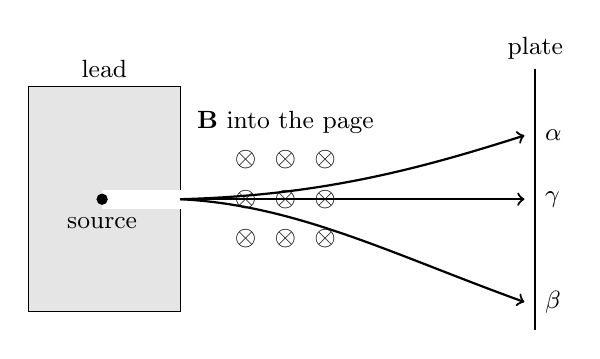
\begin{tikzpicture}[scale=0.92]
\draw[fill=gray!20] (0,-1.55) rectangle (2.1,1.55);
\draw[fill=white,draw=none] (1.02,-0.13) rectangle (2.12,0.13);
\draw[fill=black] (1.02,0) circle (0.07);
\node[below] at (1.02,-0.12) {\small source};
\node[above] at (1.05,1.55) {\small lead};
\foreach \x in {3.0,3.55,4.1}
  \foreach \y in {-0.55,0,0.55}
    \node at (\x,\y) {\(\otimes\)};
\node[above] at (3.55,0.78) {\small \(\mathbf B\) into the page};
\draw[thick] (7,-1.8) -- (7,1.8);
\node[above] at (7,1.8) {\small plate};
\draw[thick,->] (2.1,0) -- (6.85,0);
\draw[thick,->] (2.1,0) .. controls (4.0,0.05) and (5.35,0.40) .. (6.85,0.88);
\draw[thick,->] (2.1,0) .. controls (3.7,-0.08) and (5.0,-0.75) .. (6.85,-1.42);
\node[right] at (7,0.88) {\small \(\alpha\)};
\node[right] at (7,0) {\small \(\gamma\)};
\node[right] at (7,-1.42) {\small \(\beta\)};
\end{tikzpicture}
\caption{A collimated radioactive beam in a transverse magnetic field. The neutral component is undeflected, while oppositely charged components bend in opposite directions by unequal amounts.}
\end{figure}

The three components were named alpha, beta, and gamma. In modern terms,
\begin{equation}
\begin{aligned}
\beta\text{-radiation} &= \text{electrons},\\
\alpha\text{-radiation} &= \text{helium nuclei},\\
\gamma\text{-radiation} &= \text{photons}.
\end{aligned}
\end{equation}
An alpha particle contains two protons and two neutrons, explaining its mass number four. In Dalton's approximate integer sequence, helium would therefore have occupied number four: four hydrogen-scale nuclear units. Beta rays are the negatively charged electrons already known from cathode-ray experiments. Gamma rays carry no electric charge.

With a sufficiently dilute source and a detector capable of resolving individual arrivals, the continuous-looking exposure becomes a sequence of separate events: blip, blip, blip. The same can be done for beta, alpha, and gamma radiation. A Geiger counter gives the right picture, whether or not the earliest apparatus was operated in precisely that regime. Each component arrives in discrete bundles. Gamma remains the puzzle: it is neutral, yet it is detected one event at a time. Gamma radiation is very-high-energy light, and Planck and especially Einstein connected light with quanta. Before confronting that conclusion, however, the classical evidence that light is a wave has to be taken seriously.

\section{The Classical Wave Character of Light}

Classically, light was the strongest example of continuity. It consists of electric and magnetic fields propagating as continuous waves. Newton had favored a corpuscular picture, but wave experiments displaced it. Shaking a charge produces electromagnetic radiation. A macroscopic antenna can emit radio waves, microwaves, infrared, visible light, or ultraviolet radiation; a charge moving around within an atom is also an antenna. The emitted radiation can expose a photographic plate.

A single opening gives a first indication of wave behavior. If light were a stream of bullets, a small opening would be expected to make a sharply collimated spot. Instead the illumination spreads into a fuzzy region. Spreading alone is not decisive, however, because one could imagine particles being deflected by forces at the edge of the aperture.

Two openings produce the sharper test. Two independent particle streams would give two overlapping smears, perhaps brightest where they overlap. Waves do something different. A crest from one opening can meet a crest from the other and reinforce it; a crest can also meet a trough and cancel it. The screen therefore shows alternating bright and dark bands, including dark places that either opening alone would illuminate.\footnote{The schematic reconstructs the aperture and interference diagrams developed in the lecture video between 00:25:00 and 00:29:49.}

\begin{figure}[h]
\centering
\resizebox{\linewidth}{!}{%
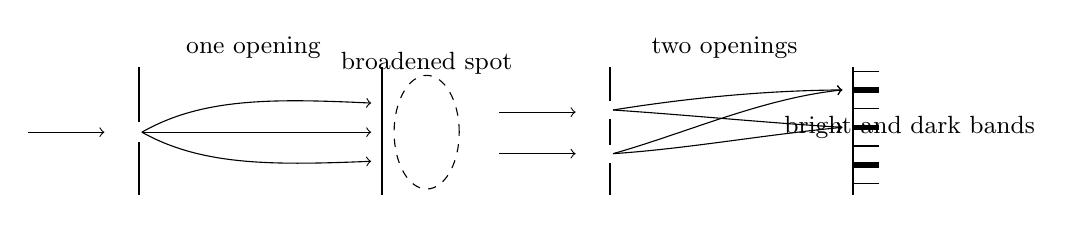
\begin{tikzpicture}[scale=0.88]
\begin{scope}
\draw[->] (-0.3,1.06) -- (0.8,1.06);
\draw[thick] (1.3,0.15) -- (1.3,0.92);
\draw[thick] (1.3,1.20) -- (1.3,2.0);
\draw[thick] (4.8,0.15) -- (4.8,2.0);
\draw[->] (1.34,1.06) .. controls (2.2,1.55) and (3.2,1.55) .. (4.65,1.48);
\draw[->] (1.34,1.06) -- (4.65,1.06);
\draw[->] (1.34,1.06) .. controls (2.2,0.58) and (3.2,0.58) .. (4.65,0.64);
\draw[dashed] (5.45,1.06) ellipse (0.47 and 0.82);
\node at (2.95,2.28) {\small one opening};
\node at (5.45,2.05) {\small broadened spot};
\end{scope}
\begin{scope}[xshift=6.8cm]
\draw[->] (-0.3,1.35) -- (0.8,1.35);
\draw[->] (-0.3,0.75) -- (0.8,0.75);
\draw[thick] (1.3,0.15) -- (1.3,0.62);
\draw[thick] (1.3,0.88) -- (1.3,1.25);
\draw[thick] (1.3,1.51) -- (1.3,2.0);
\draw[thick] (4.8,0.15) -- (4.8,2.0);
\draw[thin] (4.8,0.32) -- (5.18,0.32);
\draw[line width=2pt] (4.8,0.59) -- (5.18,0.59);
\draw[thin] (4.8,0.86) -- (5.18,0.86);
\draw[line width=2pt] (4.8,1.13) -- (5.18,1.13);
\draw[thin] (4.8,1.40) -- (5.18,1.40);
\draw[line width=2pt] (4.8,1.67) -- (5.18,1.67);
\draw[thin] (4.8,1.94) -- (5.18,1.94);
\draw[->] (1.34,0.75) .. controls (2.4,0.82) and (3.5,1.02) .. (4.65,1.13);
\draw[->] (1.34,1.38) .. controls (2.4,1.31) and (3.5,1.20) .. (4.65,1.13);
\draw[->] (1.34,0.75) .. controls (2.4,1.05) and (3.5,1.55) .. (4.65,1.67);
\draw[->] (1.34,1.38) .. controls (2.4,1.55) and (3.5,1.66) .. (4.65,1.67);
\node at (2.95,2.28) {\small two openings};
\node at (5.62,1.13) {\small bright and dark bands};
\end{scope}
\end{tikzpicture}
}
\caption{A single aperture produces a broadened image, while two apertures produce alternating constructive and destructive interference.}
\end{figure}

The same effect is easy to imagine with water. Wiggle two fingers in the surface: the circular waves spread, reinforce at some places, and cancel at others. Interference, rather than mere spreading, is the decisive wave signature.

The historical sequence is again not simple. In this schematic account Huygens is placed before Newton as an advocate of wave propagation; Thomas Young is associated with the interference demonstration; and some of Newton's own optical experiments admit a wave-interference interpretation even though he favored corpuscles. The later interference experiments established the wave character of light beyond reasonable doubt.

Maxwell then identified what oscillates. If a light wave propagates along an axis, its electric field is transverse to that axis. Its magnetic field is also transverse and is perpendicular to the electric field. The complete pattern travels at the speed of light.\footnote{The schematic reconstructs the electromagnetic-wave diagram drawn in the lecture video at 00:31:08.}

\begin{figure}[h]
\centering
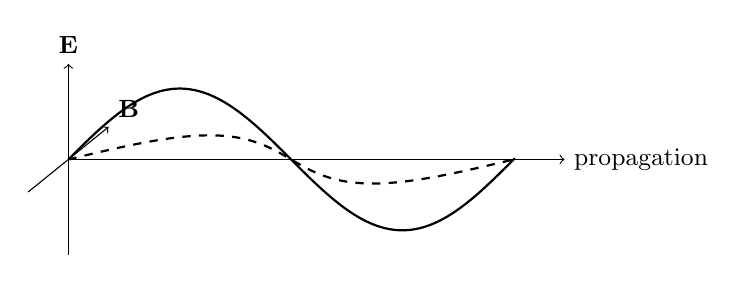
\begin{tikzpicture}[
  scale=0.9,
  x={(1cm,0cm)},
  y={(0cm,1cm)},
  z={(0.42cm,0.34cm)}
]
\draw[->] (0,0,0) -- (7,0,0) node[right] {\small propagation};
\draw[->] (0,-1.35,0) -- (0,1.35,0) node[above] {\small \(\mathbf E\)};
\draw[->] (0,0,-1.35) -- (0,0,1.35) node[above right] {\small \(\mathbf B\)};
\draw[thick,smooth,variable=\x,domain=0:6.3,samples=100]
  plot ({\x},{sin(\x r)},0);
\draw[thick,dashed,smooth,variable=\x,domain=0:6.3,samples=100]
  plot ({\x},0,{sin(\x r)});
\end{tikzpicture}
\caption{In an electromagnetic wave, the electric and magnetic fields are mutually perpendicular and both are transverse to the direction of propagation.}
\end{figure}

Ordinary visible light oscillates far too rapidly for the alternating fields to be followed directly. For an extremely long radio wave the oscillation would be correspondingly slower. In either case the same transverse-wave geometry gives interference.

\section{Wavelength, Period, and Frequency}

The wavelength \(\lambda\) is a spatial distance: begin at one point in the oscillation and move along the wave until the same phase recurs after one full cycle. It is measured in metres, centimetres, or any other unit of length.

Now stand at one position while the wave passes. The time required for one complete cycle is the period \(T\). Visible light has an extremely short period, roughly of order \(10^{-15}\,\mathrm{s}\); longer wavelength corresponds to longer period, and shorter wavelength to shorter period.

During one period a wave advances by one wavelength, so a wave of speed \(v\) obeys
\begin{equation}
v=\frac{\lambda}{T}.
\end{equation}
Water and sound waves have their own propagation speeds. For light,
\begin{equation}
c=\frac{\lambda}{T}.
\end{equation}
The frequency \(f\) is the number of cycles per unit time:
\begin{equation}
f=\frac{1}{T}.
\end{equation}
Hence
\begin{equation}
\lambda f=c.
\end{equation}
Either wavelength or frequency determines the other.

\begin{figure}[h]
\centering

\includegraphics[width=0.68\textwidth]{lecture_01_figure_03.png}
\caption{For a light wave, \(f=1/T\) and \(\lambda f=c\).}
\lectureframe{00:36:24}
\end{figure}

Physicists often measure oscillation rate in radians per second rather than complete cycles per second. Imagine uniform motion around a circle. If the point completes \(f\) circuits each second and each circuit contains \(2\pi\) radians, its angular frequency is
\begin{equation}
\omega=2\pi f,
\qquad
\frac{\omega}{2\pi}=f.
\end{equation}
For now this is a definition; the practical question of whether it reduces the number of factors of \(2\pi\) returns later.

Combining \(f=c/\lambda\) with \(\omega=2\pi f\) gives
\begin{equation}
\omega=\frac{2\pi c}{\lambda},
\qquad
\omega\lambda=2\pi c.
\end{equation}
For another kind of wave, \(c\) is replaced by that wave's propagation speed.

\begin{figure}[h]
\centering

\includegraphics[width=0.68\textwidth]{lecture_01_figure_04.png}
\caption{With \(\omega=2\pi f\), a light wave satisfies \(\omega=2\pi c/\lambda\).}
\lectureframe{00:39:10}
\end{figure}

Electromagnetic radiation forms a continuous spectrum. Ordered from longer to shorter wavelength, the conventional names are
\begin{equation}
\begin{aligned}
\text{radio}
&\longrightarrow \text{microwave}
\longrightarrow \text{infrared}
\longrightarrow \text{visible}\\
&\longrightarrow \text{ultraviolet}
\longrightarrow \text{X ray}
\longrightarrow \text{gamma ray}.
\end{aligned}
\end{equation}
Visible light occupies only a narrow interval. The boundaries between the named regions are conventional, so no exact dividing wavelengths are needed here. Radio waves may be extremely long; gamma radiation is the very-short-wavelength end of the electromagnetic spectrum. The difficulty is now sharp: gamma radiation is classically a continuous field wave, yet it is detected in discrete blips.

\section{Discrete Arrivals and Wave Probabilities}

Thermodynamic properties of radiation led Planck and Einstein to the conclusion that light must be treated in discrete units. An imagined experiment makes the point vivid, but it is not a claim about the actual historical route to the discovery.

Shine a beam on a screen. At ordinary intensity it makes a continuous-looking illuminated blob. Put a partly opaque attenuator in the beam: the blob becomes dimmer. Increase the attenuation repeatedly and less light arrives per unit time. Eventually the appearance changes. Instead of a continuously dim blob, the detector records isolated events.\footnote{The schematic reconstructs the attenuation experiment developed in the lecture video between 00:42:32 and 00:45:42.}

\begin{figure}[h]
\centering
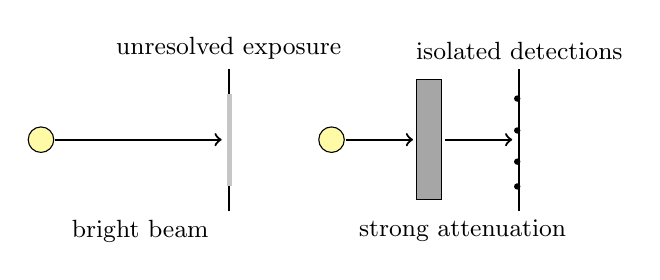
\begin{tikzpicture}[scale=0.9]
\begin{scope}
\draw[fill=yellow!35] (0,0) circle (0.18);
\draw[->,thick] (0.2,0) -- (2.55,0);
\draw[thick] (2.65,-1.0) -- (2.65,1.0);
\node[below] at (1.4,-1.0) {\small bright beam};
\end{scope}
\begin{scope}[xshift=4.1cm]
\draw[fill=yellow!35] (0,0) circle (0.18);
\draw[->,thick] (0.2,0) -- (1.15,0);
\draw[fill=gray!70] (1.2,-0.85) rectangle (1.55,0.85);
\draw[->,thick] (1.6,0) -- (2.55,0);
\draw[thick] (2.65,-1.0) -- (2.65,1.0);
\node[below] at (1.85,-1.0) {\small strong attenuation};
\end{scope}
\fill[gray!45] (2.62,-0.65) rectangle (2.70,0.65);
\foreach \y in {-0.66,-0.31,0.13,0.58}
  \fill (6.72,\y) circle (0.045);
\node[above] at (2.65,1.0) {\small unresolved exposure};
\node[above] at (6.75,1.0) {\small isolated detections};
\end{tikzpicture}
\caption{Progressive attenuation lowers the detection rate until a continuous-looking exposure resolves into isolated photon events.}
\end{figure}

Wait long enough and those events accumulate into the same spatial profile as the original blob. The bright region was therefore the unresolved sum of many individual arrivals. This low-intensity experiment can be performed, though it was not the early experiment that originally motivated the photon hypothesis. Einstein's photon proposal arose from thermodynamic and photoelectric considerations; the attenuation experiment supplies an especially direct way to picture its consequence.

Now place two apertures in the beam and reduce the intensity until photons arrive one at a time. Each detection is a localized blip. Yet after many detections the blips fill in an interference pattern, including bright and dark bands. The discrete arrivals are random, but their probability distribution is the distribution predicted by the wave pattern. The classical wave has become a wave governing probabilities.

Wave and particle are therefore not two separate kinds of entity assigned to different parts of nature. They are two manifestations of the same quantum object. Light cannot be described adequately as only a wave or only a particle.

Electrons reverse the original surprise. Electrons were accepted as particles and arrive at a detector one at a time, but with sufficiently close apertures they also build an interference pattern. Alpha particles, about eight thousand times heavier than electrons, obey the same principle, although the experiment is harder. Interference has even been observed with buckyballs: molecules of sixty carbon atoms arranged approximately like a generalized soccer ball. The same principle is expected to apply even to bowling balls, although such an experiment is fantastically impractical. The discussion can be pushed toward proposed experiments with viruses or living cells as increasingly ambitious examples. Understanding how wave and particle descriptions fit together requires quantum mechanics; the immediate task is to extract the photon properties needed for particle physics.

\section{Photon Energy}

Photons are the discrete, indivisible elements of light. Light carries energy---sunlight heats an absorbing object---so each photon must carry energy. A monochromatic wave has a definite wavelength and angular frequency, and every photon in it has
\begin{equation}
E_\gamma=\hbar\omega.
\end{equation}
Trying to picture a continuous wave as a little mechanical collection of dots is misleading. What is definite is the experimental combination: localized detections occur with a wave-governed distribution, and the energy arrives in indivisible units.

Since
\begin{equation}
\omega=\frac{2\pi c}{\lambda},
\end{equation}
a shorter wavelength means a larger angular frequency and therefore more energy in each photon:
\begin{equation}
\lambda\downarrow
\quad\Longrightarrow\quad
\omega\uparrow
\quad\Longrightarrow\quad
E_\gamma\uparrow.
\end{equation}
A single radio photon has very little energy. A radio beam can nevertheless carry enormous total energy by containing very many photons. For a monochromatic pulse containing \(n\) photons,
\begin{equation}
E_{\text{pulse}}=n\hbar\omega,
\qquad
n=0,1,2,\ldots.
\end{equation}
The total may be large, but it remains an integer multiple of the one-photon energy.

This relation points toward the practical question that will govern the rest of the discussion. Why must bigger and bigger machines be built to see smaller and smaller things? Why not use a small machine for a small object? The first half of the answer is already present: resolving smaller structure requires shorter wavelength, and a shorter-wavelength quantum carries greater energy.

\section{Rest Energy and Invariant Mass}

Particle physics combines quantum mechanics with relativity. The photon relation \(E_\gamma=\hbar\omega\) supplies the quantum side; the corresponding elementary fact from relativity is
\begin{equation}
E_{\mathrm{rest}}=mc^2.
\end{equation}
The qualification matters. Older accounts distinguished \emph{rest mass} from a velocity-dependent \emph{moving mass}. Modern terminology uses \emph{mass} for the invariant mass of an object. Motion changes its energy, not its mass. Every electron has the same mass, whatever its state of motion, while an electron's energy increases as it is accelerated. Thus \(E=mc^2\), in this form, is the energy of a massive object in a frame in which the object as a whole is at rest.

The object need not be internally motionless. A box of gas can stand still on a scale while its molecules move rapidly in all directions. The energy of those internal motions is part of the rest energy of the complete box. Begin with a cold box, measure its mass, and then add thermal energy while keeping the box itself at rest. Its rest mass changes by
\begin{equation}
\Delta m=\frac{\Delta E_{\mathrm{internal}}}{c^2}.
\end{equation}
Its weight and inertia increase with its mass. For an ordinary box, even after a large temperature increase, the effect is far too small to notice on an ordinary scale; the smallness of the effect does not change the principle.

A sharper example uses an electron and a positron. They have precisely equal masses and opposite electric charges. If they are initially at rest and annihilate, photons carry away the energy:
\begin{equation}
e^-+e^+\longrightarrow \text{photons}.
\end{equation}
The initial energy is
\begin{equation}
E_{\mathrm{initial}}=2m_e c^2,
\end{equation}
and that energy cannot disappear. A single pair yields only a tiny amount, so enormous numbers of pairs would be needed to heat even a cup of coffee, but individual annihilation events exhibit the conversion directly.

For an object at rest, mass and energy are therefore the same physical quantity expressed in different units. The factor \(c^2\) is the conversion factor between the customary mass and energy units, much as a numerical factor converts metres to centimetres.

\begin{classroomqa}
\lecturetimestamp{01:04:39}
\audiencequestion{Does converting mass into released energy require a mechanism?}
\lecturerresponse{Yes, a physical mechanism is required, but conservation laws already constrain its outcome. Even before the microscopic annihilation mechanism is described, the initial electron--positron energy must reappear somewhere. Conservation of energy can therefore determine an important part of the answer without a detailed account of the interaction.}
\end{classroomqa}

\section{Dimensions and the Choice of Units}

In SI units the speed of light is a very large number and Planck's constant is a very small one. The smallness of the latter is already suggested by the photon relation: the angular frequency of visible light is enormous while the energy of one photon is tiny, so \(E_\gamma=\hbar\omega\) requires a small numerical value of \(\hbar\) in these units. At the level of order of magnitude,
\begin{equation}
c\sim 10^8\ \mathrm{m\,s^{-1}},
\qquad
\hbar\sim 10^{-34}\ \mathrm{J\,s}.
\end{equation}
\editorialnote{Only the orders of magnitude stated in the lecture are retained because the final board digits are indistinct.}
Units are essential: neither constant is merely a bare decimal. Since energy has the dimensions
\begin{equation}
[E]=M L^2 T^{-2},
\end{equation}
and \(E_\gamma=\hbar\omega\) with \([\omega]=T^{-1}\), Planck's constant has dimensions
\begin{equation}
[\hbar]=[E]T=M L^2 T^{-1}.
\end{equation}

Calling \(c\) large and \(\hbar\) small already presupposes a choice of units. Measuring speed in feet per hour produces a different numerical value of \(c\) from measuring it in metres per second. In light-years per year, or light-seconds per second, the speed of light is simply one. A suitable coordinated choice of mass, length, and time units can likewise make \(\hbar=1\).

Familiar systems of units are inherited conventions, not privileged features of nature. A mile contains 5280 feet, a stone contains fourteen pounds, horses are measured in hands, and power may be measured in horsepower. Metric units are more systematic, but their scales remain human choices. Nothing in fundamental physics singles out the metre, second, or kilogram.

Length, time, and mass provide three independent basic unit choices:
\begin{equation}
L,\qquad T,\qquad M.
\end{equation}
Other mechanical units can be built from them. The useful choices depend on the problem. A solar mass is convenient in astrophysics; a proton mass may be convenient in nuclear physics; light-years and years make relativistic astronomical formulas compact. With three independent choices, one can assign convenient numerical values to three independent dimensional constants. Astrophysics, atomic physics, and particle physics need not make the same choices.

For particle physics, two particularly useful conventions are
\begin{equation}
c=1,
\qquad
\hbar=1.
\end{equation}
There is no comparably distinguished particle mass for the remaining unit. One could declare the proton mass, Higgs-boson mass, or muon mass to be one, but that would merely privilege one member of a large collection.

Why choose \(c\) and \(\hbar\), then? A first answer might be that they appear in many equations. Frequency of appearance is not enough: the proton mass also appears in many equations, and so does the proton's size. What distinguishes \(c\) and \(\hbar\) is their universality.

The constants \(c\) and \(\hbar\) are different. The speed \(c\) constrains every physical object: massive objects may approach it but cannot be accelerated through it. Planck's constant constrains every quantum object through the order-of-magnitude uncertainty relation
\begin{equation}
\Delta x\,\Delta p\gtrsim\hbar.
\end{equation}
Neither statement singles out a particular species of particle. This universality is what makes \(c=1\) and \(\hbar=1\) natural conventions.

The proton supplies no comparable universal scale. It is only one object among many. Setting the proton mass to one would have no more fundamental standing than setting the mass of a rubidium atom to one; the electron, Higgs boson, and muon present the same difficulty.

Electric charge suggests another universal quantity, but after \(c\) and \(\hbar\) have been normalized, the physically significant electromagnetic coupling is dimensionless. Changing units can move dimensional constants around an electromagnetic formula; it cannot change a genuine dimensionless coupling.

Gravity supplies a dimensional universal constant. In Newtonian form, the magnitude of the force between two masses is
\begin{equation}
F=G\frac{m_1m_2}{r^2}.
\end{equation}
Every mass gravitates, whereas electrically neutral objects need not participate in an electric force. Thus \(G\) has the required universality. It is nevertheless a poor practical normalization for ordinary particle physics because gravitational forces between known elementary particles are negligible in the calculations under discussion.

\begin{classroomqa}
\lecturetimestamp{01:20:34}
\audiencequestion{Is it legitimate simply to dismiss \(G\)? At very high energies, elementary particles might not obey classical gravity in the way being assumed.}
\lecturerresponse{Individual particles do respond to the Earth's gravitational field: a single particle falls in that field. The gravitational influence of one elementary particle on another has not been measured directly, so the universality assumption can be questioned at that level. The immediate reason for leaving \(G\) out is practical rather than absolute: gravity contributes negligibly to ordinary particle-physics experiments and equations.}
\end{classroomqa}

\begin{classroomqa}
\lecturetimestamp{01:22:01}
\audiencequestion{Could the electric interaction be used as the third unit-setting convention instead of gravity?}
\lecturerresponse{Yes. One can choose electromagnetic units in which electric charge, or the constant appearing in Coulomb's law, is normalized. Such conventions are used. Electrons repel rather than attract, but that sign does not obstruct the choice. It is simply not the convention adopted here.}
\end{classroomqa}

\begin{classroomqa}
\lecturetimestamp{01:23:06}
\audiencequestion{Once \(c\) and \(\hbar\) are set equal to one, is electric charge dimensionless?}
\lecturerresponse{Yes. A dimensionless measure associated with the square of the electric charge is approximately \(1/137\). The precise convention and the meaning of that number can be postponed; the point here is that it is dimensionless.}
\end{classroomqa}

\begin{classroomqa}
\lecturetimestamp{01:23:37}
\audiencequestion{Could Coulomb's constant be chosen as the third constant set equal to one?}
\lecturerresponse{It can be absorbed into the electromagnetic unit convention. That choice cannot turn the dimensionless coupling \(1/137\) into one, because changing units cannot alter a dimensionless number. No particular benefit is claimed for adopting that convention here.}
\end{classroomqa}

\section{Natural-Unit Equations and Reference Frames}

With \(c=1\), the rest-energy relation for a massive object becomes
\begin{equation}
E_{\mathrm{rest}}=m.
\end{equation}
With \(\hbar=1\), the photon relation becomes
\begin{equation}
E_\gamma=\omega.
\end{equation}
The constants can be restored whenever numerical sizes in conventional units are needed.

\begin{figure}[h]
\centering

\includegraphics[width=0.72\textwidth]{lecture_01_figure_05.png}
\caption{In units with \(c=1\), the rest energy of a massive object at rest is \(E=m\).}
\lectureframe{01:25:40}
\end{figure}

These formulas look similar but mean different things. In \(E_{\mathrm{rest}}=m\), \(E\) is the rest energy of a massive object. A photon has no mass and cannot be brought to rest, so its energy is not rest energy. The relation \(E_\gamma=\omega\) gives the energy of a moving, massless quantum.

\begin{classroomqa}
\lecturetimestamp{01:26:07}
\audiencequestion{What does \emph{at rest} mean when rest is always relative to something and the laboratory itself is not absolutely at rest?}
\lecturerresponse{Rest is defined relative to a chosen frame. If a cup is stationary relative to the laboratory, then in that laboratory frame its energy is its mass when \(c=1\), with no overall kinetic contribution. Another observer moving past the cup assigns it kinetic energy as well. Different observers generally assign different energies to the same object or photon; energy is frame-dependent, and no claim of absolute rest is required.}
\end{classroomqa}

The angular-frequency convention can now be reconsidered. Writing \(E_\gamma=\hbar\omega\) is compact, but \(\omega=2\pi f\) inserted a factor of \(2\pi\) earlier.

\begin{classroomqa}
\lecturetimestamp{01:28:13}
\audiencequestion{Why use angular frequency \(\omega\), measured in radians per second, rather than the apparently simpler number of complete cycles per second?}
\lecturerresponse{The choice is partly historical, and the mathematical answer is pragmatic rather than immediate. The answer offered here is tentative: write the relevant equations once with \(f\) and once with \(\omega\), then see which convention leaves fewer factors of \(2\pi\). The factors of \(2\pi\) cannot be made to disappear everywhere. A possible connection with complex-exponential notation was also suggested, but it is not developed here.}
\end{classroomqa}

\begin{classroomqa}
\lecturetimestamp{01:29:51}
\audiencequestion{Can two particles be accelerated until their mutual gravitational interaction becomes important?}
\lecturerresponse{In principle, yes. In practice, present accelerators are extraordinarily far from that regime. The answer also depends on what is meant by a particle: a macroscopic gravitating body is not the elementary-particle case at issue.}
\end{classroomqa}

\begin{classroomqa}
\lecturetimestamp{01:30:27}
\audiencequestion{What can serve as a source of positrons?}
\lecturerresponse{High-energy collisions can create positrons. Some nuclear processes and decays produce them as well.}
\end{classroomqa}

\begin{classroomqa}
\lecturetimestamp{01:30:53}
\audiencequestion{Are Planck time and Planck distance the natural units being used here?}
\lecturerresponse{No. Planck units arise when \(G\), \(c\), and \(\hbar\) are all set equal to one. The resulting Planck length is far smaller than the length scales of ordinary particle physics, so it is an inconvenient measuring stick here. Such units are natural when gravity, quantum mechanics, and relativity all matter together, as in black-hole physics, cosmology, or quantum gravity. When gravity is negligible, setting only \(c\) and \(\hbar\) equal to one is more useful.}
\end{classroomqa}

\section{Momentum, Light, and Resolution}

The next basic concept is momentum. An object at rest has no momentum, even though it has the nonzero rest energy \(mc^2\). Once it moves, it generally carries momentum. Momentum is conserved in a collision just as energy is conserved: when two objects collide, the total vector momentum before and after the collision is the same. Anything constrained by a conservation law deserves special attention.

Momentum is a vector: it points along the direction of motion. For a nonrelativistic object,
\begin{equation}
\mathbf p=m\mathbf v.
\end{equation}
This is not the general relativistic formula, and it cannot be applied directly to light.

Light nevertheless carries momentum as well as energy. Ordinary light produces so little push that its momentum is hard to notice, but an intense laser pulse can transfer a substantial impulse. The large laser at Livermore, for example, can drive material inward with the momentum carried by its radiation.

Consider a pulse sufficiently well collimated that its rays travel nearly along one axis. A real beam may have some angular spread, with portions traveling in slightly different directions, but for an ideal collimated beam the momentum points along the beam and has magnitude
\begin{equation}
p=\frac{E}{c},
\qquad\text{or equivalently}\qquad
E=cp.
\end{equation}
This relation is taken as a relativistic fact here rather than proved. The following dimensional check only confirms that its units agree with those of ordinary momentum:
\begin{equation}
\left[\frac{E}{c}\right]
=
\frac{M L^2 T^{-2}}{L T^{-1}}
=
M L T^{-1}
=
[m v]
=
[p].
\end{equation}
This dimensional comparison does not assign a rest mass to light. A photon has zero mass; it carries momentum because it carries energy and moves at \(c\).

The direction of \(\mathbf p\) is the direction of propagation. Its magnitude is usually difficult to detect because \(c\) appears in the denominator. A beam can readily reveal its energy by heating or evaporating matter, while its mechanical push is much smaller. With enough intensity, however, that push can become large.

For one photon,
\begin{align}
p_\gamma
&=\frac{E_\gamma}{c}\\
&=\frac{\hbar\omega}{c}.
\end{align}
To express this in terms of wavelength, return carefully to the wave relations. Since
\begin{equation}
f\lambda=c,
\qquad
\omega=2\pi f,
\end{equation}
the correct relation is
\begin{equation}
\omega\lambda=2\pi c,
\qquad
\omega=\frac{2\pi c}{\lambda}.
\end{equation}
The factor of \(2\pi\) is easy to reverse if the definitions are not written out. Starting again from \(f\lambda=c\) and \(f=\omega/(2\pi)\) settles the issue:
\begin{equation}
\frac{\omega}{2\pi}\lambda=c
\quad\Longrightarrow\quad
\omega\lambda=2\pi c.
\end{equation}
Substitution now gives
\begin{align}
p_\gamma
&=\frac{\hbar}{c}\frac{2\pi c}{\lambda}\\
&=\frac{2\pi\hbar}{\lambda}\\
&=\frac{h}{\lambda}.
\end{align}

\begin{classroomqa}
\lecturetimestamp{01:42:38}
\audiencequestion{Is \(2\pi\hbar\) equal to \(h\)?}
\lecturerresponse{Yes. By definition \(h=2\pi\hbar\), so \(p_\gamma=2\pi\hbar/\lambda\) is the same as \(p_\gamma=h/\lambda\). Factors of \(2\pi\) reappear somewhere whichever frequency convention is chosen.}
\end{classroomqa}

The shorter the wavelength, the larger the photon momentum. A radio photon has a very long wavelength and a tiny momentum. A gamma-ray photon has a very short wavelength and a much larger kick. One photon still gives only a small macroscopic impulse, but its momentum is much larger than that of a radio photon. Its energy is larger as well, since \(E_\gamma=cp_\gamma\).

This relation explains why smaller objects require larger machines. A photograph made with wavelengths much longer than a person's head could show only a blur. To distinguish facial features, the wavelength must be shorter than the head. To resolve one hair, it must be comparable to or smaller than the hair's thickness. To resolve the structure of an atom, the probe wavelength must be no larger than the atom:
\begin{equation}
\lambda_{\mathrm{probe}}\lesssim
\text{size of the structure to be resolved}.
\end{equation}
Smaller structures therefore require shorter wavelengths, and shorter wavelengths require larger momentum and energy. The probe need not be a photon; high-energy particles of other kinds obey the same quantum connection between wavelength and momentum. Producing them requires accelerators that transfer more and more energy to each particle. The pair \(p_\gamma=h/\lambda\) and \(E_\gamma=\hbar\omega\) carries the argument: increasing the probe energy increases its momentum and shortens its wavelength.

This has been the recurring pattern of particle physics for roughly a century: higher energy, larger momentum, shorter wavelength, and finer spatial resolution.

\begin{classroomqa}
\lecturetimestamp{01:46:57}
\audiencequestion{Is there a theoretical lower limit to wavelength?}
\lecturerresponse{Possibly. Something new is expected near the Planck length, but the answer is tentative. If spatial resolution bottoms out there, that scale is still about seventeen orders of magnitude below the distances being probed at the LHC, so present experiments remain enormously far from it.}
\end{classroomqa}

The same chain of reasoning suggests a rough connection between the scale of an accelerator and the scale it can resolve.

\begin{classroomqa}
\lecturetimestamp{01:48:02}
\audiencequestion{Is the wavelength, or the size being resolved, roughly inversely related to the size of the accelerator?}
\lecturerresponse{Roughly, yes, provided the maximum electric fields that accelerate the particles, and the magnetic fields used to guide them, remain fixed by the available apparatus. An accelerating gradient is an energy gain per unit length. For a linear accelerator of length \(L\) and approximately fixed gradient \(\mathcal G\),
\[
E_{\mathrm{beam}}\sim \mathcal G L.
\]
At ultrarelativistic energies the resolvable wavelength is inversely related to energy, so increasing the linear accelerator's length improves the resolution by roughly the inverse factor. This is only a heuristic scaling, not an exact law. Circular machines allow the same apparatus to be traversed repeatedly, but accelerated charges radiate while bending and lose energy.}
\end{classroomqa}

\begin{classroomqa}
\lecturetimestamp{01:49:47}
\audiencequestion{How large would an accelerator have to be to reach the Planck length?}
\lecturerresponse{On this rough scaling, it would have to be about seventeen orders of magnitude longer than CERN's accelerator. That is not the size of the universe, but it is roughly galactic in scale.}
\end{classroomqa}

\begin{classroomqa}
\lecturetimestamp{01:50:09}
\audiencequestion{How do the energies of the highest-energy cosmic rays compare with collider energies?}
\lecturerresponse{Individual cosmic rays can have far more laboratory energy. For the numerical comparison, take an extreme cosmic ray with laboratory energy of order \(10^{21}\,\mathrm{eV}=10^{12}\,\mathrm{GeV}\). But a cosmic ray strikes a target that is stationary in the laboratory, whereas a collider brings two energetic beams together head-on. More importantly, useful experiments require flux: many particles and many well-controlled collisions. A lone cosmic ray may miss the relevant target or produce an event from which little can be inferred. An intentionally extravagant oil-equivalent estimate put the supply needed to run a useful galactic accelerator at about one hundred trillion barrels of oil per second. Its purpose is to show that adequate collision statistics would be at least as serious an obstacle as the accelerator's length.}
\end{classroomqa}

\editorialnote{The oil-equivalent estimate is inconsistent in the source. It is first stated and then repeated as about \(10^{14}\) barrels per second; a later restatement gives \(10^{11}\) barrels per second. Both scales are retained rather than silently reconciled.}

These are real distance scales, not merely formal ones. The practical puzzle is how to probe them without constructing a galactic accelerator and supplying its fantastical power.

\begin{classroomqa}
\lecturetimestamp{01:52:55}
\audiencequestion{How should the LHC energy be compared with a cosmic ray of energy \(10^{12}\,\mathrm{GeV}\)?}
\lecturerresponse{For an ultrarelativistic projectile of laboratory energy \(E_{\mathrm{lab}}\) striking a fixed target of mass \(m_{\mathrm{target}}\), the center-of-mass energy behaves parametrically as
\[
E_{\mathrm{cm}}\simeq
\sqrt{2m_{\mathrm{target}}c^2E_{\mathrm{lab}}}.
\]
\editorialnote{The displayed fixed-target expression makes explicit the square-root scaling stated in the exchange.}
With the target mass held fixed, the useful collision energy therefore grows only as the square root of the projectile energy. Thus a \(10^{12}\,\mathrm{GeV}\) cosmic ray corresponds, at order-of-magnitude level, to counter-propagating beam energies of order \(10^6\,\mathrm{GeV}\) per beam, not \(10^{12}\,\mathrm{GeV}\) in each beam. Cosmic rays can still exceed terrestrial collider energies, but their very low flux makes systematic, controlled experiments impractical.}
\end{classroomqa}
